\documentclass{article}
\usepackage[greek,english]{babel}
\usepackage[utf8]{inputenc}
\usepackage{alphabeta}
\usepackage{graphicx}

\begin{document}
% \sffamily
% \ttfamily

\title{E - Broker: Μια λεπτομερής ανάλυση}
\author{
	Ιωάννης Χείλαρης - 1115201500176
	\\
	Ιωάννης Μαλιάρας - 1115201500084
}

\maketitle

\newpage
\tableofcontents


\newpage
\section{Εισαγωγή}
	Στα πλαίσια αυτής της εργασίας, θα σχεδιάσουμε μια εφαρμογή Ιστού για τη διαβίβαση εντολών αγοράς και πώλησης μετοχών μιας εταιρίας.
	Αρχικά, θα μελετήσουμε τις απαιτήσεις του παραπάνω συστήματος με τη χρήση μεθόδων δομημένης ανάλυσης.

	
\newpage
\section{Δομημένη Ανάλυση}
	\subsection{Γενικό Διάγραμμα Ροής Δεδομένων}

		\subsection*{Παραδοχές}
		\begin{itemize}
			\item Το ΧΑΑ προμηθεύει το σύστημα E-Broker με όλα τα δεδομένα των μετοχών που διατίθενται προς αγοραπωλησία.
			\item Το ΧΑΑ ενημερώνει το σύστημα E-Broker περί της διαθεσιμότητας του (σε περίπτωση αργίας), αλλά και όλων των μετοχών που διατίθεται προς αγοραπωλησία
		\end{itemize}

		Τα 2 παραπάνω συνοψίζονται στο βέλος "Δεδομένα Μετοχών".

		\begin{figure}[!h]
			
\includegraphics[width=\linewidth]{../Structured_Analysis/General_Diagram.png}
		\end{figure}
	
	\newpage
	\subsection{Διάγραμμα Ροής Δεδομένων Επιπέδου 1}
	\subsection*{Παραδοχές}
	\begin{itemize}
		\item Θεωρούμε οτι η διαδικασία διαχείρισης εντολών είναι αυτή που ενημερώνει τον πελάτη για απόρριψη εντολών μετά την αρχική αποδοχή τους από το ΧΑΑ.
		Αυτή η λειτουργία συνοψίζεται από τις ροές δεδομένων "Αποδοχή/Απόρριψη" και "Ενημέρωση Κατάστασης Εντολής".
	\end{itemize}

	\begin{figure}[!h]
		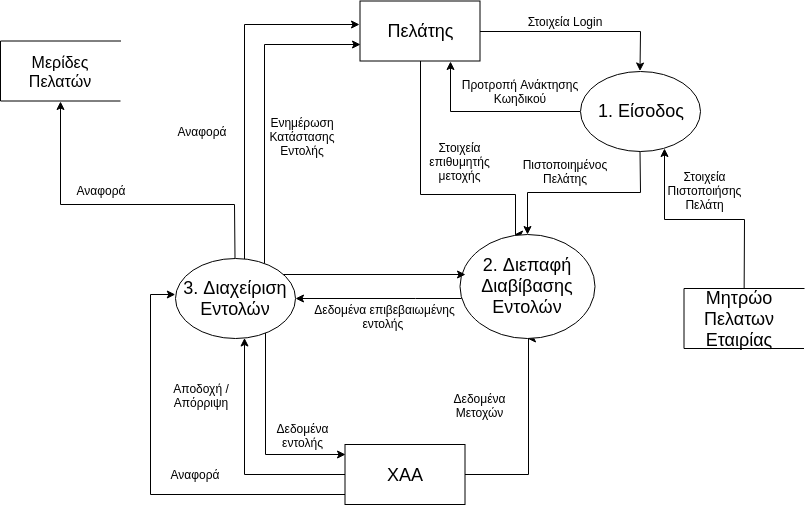
\includegraphics[width=\linewidth]{../Structured_Analysis/Level_1_Diagram.png}
	\end{figure}

	\newpage
	\subsection{Διάγραμμα Ροής Δεδομένων Επιπέδου 2}
	\subsection*{Παραδοχές}
	\begin{itemize}
		\item 3.1 Επεξεργασία εντολής: 
			\begin{itemize}
				\item Ανάλυση εντολής.
				\item Πιστοποίηση πληρότητας στοιχείων χρήστη.
			\end{itemize}
		
		\item 3.2 Πληρωμή
			\begin{itemize}
				\item Διεκπεραίωση συναλλαγής με την τράπεζα.
			\end{itemize}

		\item 3.3 Επικοινωνία ΧΑΑ:
			\begin{itemize}
				\item Αποστολή εντολής στο ΧΑΑ.
				\item Συλλογή απόκρισης (Αποδοχή / Απόρριψη) από ΧΑΑ.
				\item Συλλογή αναφοράς εκκαθάρισης.
				\item Διαβίβαση πληροφορίας σε άλλες διεργασίες και σε πελάτη.
			\end{itemize}

		\item 3.4 Ενημέρωση Μερίδων:
		\begin{itemize}
			\item Υπολογισμός προμήθειας και λοιπών οικονομικών στοιχείων.
			\item Ενημέρωση μερίδας τίτλων πελάτη.
			\item Ενημέρωση ταμειακής μερίδας πελάτη.
		\end{itemize}
	\end{itemize}

	\begin{figure}[!h]
		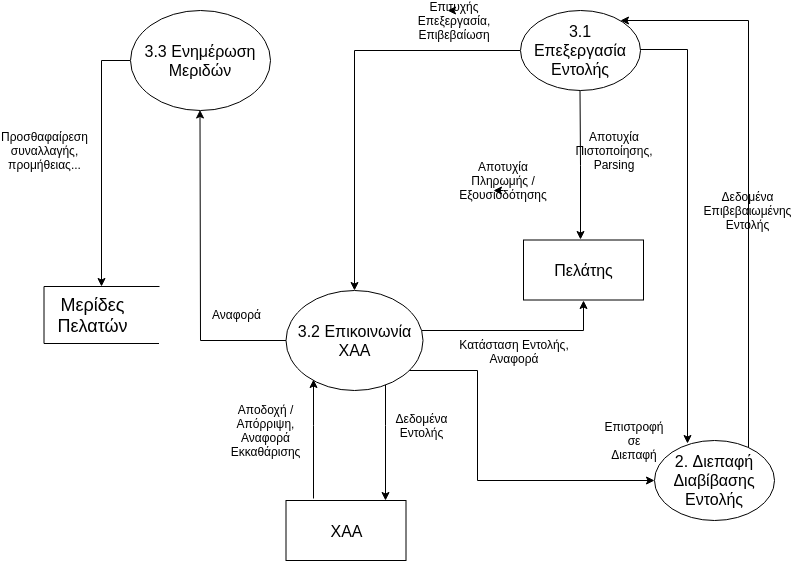
\includegraphics[width=\linewidth]{../Structured_Analysis/Level_2_Diagram.png}
	\end{figure}

\newpage
\section{Επίλογος}



\end{document}